\documentclass[11pt]{article}

\newcommand{\yourname}{Zerun Tian}
\newcommand{\yourcollaborators}{}

\def\comments{0}
\setlength{\parindent}{0 in}
\setlength{\parskip}{0.1in}

%format and packages

%\usepackage{algorithm, algorithmic}
\usepackage[noend]{algpseudocode}
\usepackage{amsmath, amssymb, amsthm}
\usepackage{enumerate}
\usepackage{enumitem}
\usepackage{framed}
\usepackage{verbatim}
\usepackage[margin=1.0in]{geometry}
\usepackage{microtype}
\usepackage{kpfonts}
\usepackage{palatino}
	\DeclareMathAlphabet{\mathtt}{OT1}{cmtt}{m}{n}
	\SetMathAlphabet{\mathtt}{bold}{OT1}{cmtt}{bx}{n}
	\DeclareMathAlphabet{\mathsf}{OT1}{cmss}{m}{n}
	\SetMathAlphabet{\mathsf}{bold}{OT1}{cmss}{bx}{n}
	\renewcommand*\ttdefault{cmtt}
	\renewcommand*\sfdefault{cmss}
	\renewcommand{\baselinestretch}{1.06}
\usepackage[usenames,dvipsnames]{xcolor}
\definecolor{DarkGreen}{rgb}{0.15,0.5,0.15}
\definecolor{DarkRed}{rgb}{0.6,0.2,0.2}
\definecolor{DarkBlue}{rgb}{0.2,0.2,0.6}
\definecolor{DarkPurple}{rgb}{0.4,0.2,0.4}
\usepackage[pdftex]{hyperref}
\hypersetup{
	linktocpage=true,
	colorlinks=true,				% false: boxed links; true: colored links
	linkcolor=DarkBlue,		% color of internal links
	citecolor=DarkBlue,	% color of links to bibliography
	urlcolor=DarkBlue,		% color of external links
}

\usepackage{graphicx}
\graphicspath{ {./} }

%enclosure macros
\newcommand{\paren}[1]{\ensuremath{\left( {#1} \right)}}
\newcommand{\bracket}[1]{\ensuremath{\left\{ {#1} \right\}}}
\renewcommand{\sb}[1]{\ensuremath{\left[ {#1} \right\]}}
\newcommand{\ab}[1]{\ensuremath{\left\langle {#1} \right\rangle}}

%probability macros
\newcommand{\ex}[2]{{\ifx&#1& \mathbb{E} \else \underset{#1}{\mathbb{E}} \fi \left[#2\right]}}
\newcommand{\pr}[2]{{\ifx&#1& \mathbb{P} \else \underset{#1}{\mathbb{P}} \fi \left[#2\right]}}
\newcommand{\var}[2]{{\ifx&#1& \mathrm{Var} \else \underset{#1}{\mathrm{Var}} \fi \left[#2\right]}}

%useful CS macros
\newcommand{\poly}{\mathrm{poly}}
\newcommand{\polylog}{\mathrm{polylog}}
\newcommand{\zo}{\{0,1\}}
\newcommand{\pmo}{\{\pm1\}}
\newcommand{\getsr}{\gets_{\mbox{\tiny R}}}
\newcommand{\card}[1]{\left| #1 \right|}
\newcommand{\set}[1]{\left\{#1\right\}}
\newcommand{\negl}{\mathrm{negl}}
\newcommand{\eps}{\varepsilon}
\DeclareMathOperator*{\argmin}{arg\,min}
\DeclareMathOperator*{\argmax}{arg\,max}
\newcommand{\eqand}{\qquad \textrm{and} \qquad}
\newcommand{\ind}[1]{\mathbb{I}\{#1\}}
\newcommand{\sslash}{\ensuremath{\mathbin{/\mkern-3mu/}}}

%mathbb
\newcommand{\N}{\mathbb{N}}
\newcommand{\R}{\mathbb{R}}
\newcommand{\Z}{\mathbb{Z}}
%mathcal
\newcommand{\cA}{\mathcal{A}}
\newcommand{\cB}{\mathcal{B}}
\newcommand{\cC}{\mathcal{C}}
\newcommand{\cD}{\mathcal{D}}
\newcommand{\cE}{\mathcal{E}}
\newcommand{\cF}{\mathcal{F}}
\newcommand{\cL}{\mathcal{L}}
\newcommand{\cM}{\mathcal{M}}
\newcommand{\cO}{\mathcal{O}}
\newcommand{\cP}{\mathcal{P}}
\newcommand{\cQ}{\mathcal{Q}}
\newcommand{\cR}{\mathcal{R}}
\newcommand{\cS}{\mathcal{S}}
\newcommand{\cU}{\mathcal{U}}
\newcommand{\cV}{\mathcal{V}}
\newcommand{\cW}{\mathcal{W}}
\newcommand{\cX}{\mathcal{X}}
\newcommand{\cY}{\mathcal{Y}}
\newcommand{\cZ}{\mathcal{Z}}

%theorem macros
\newtheorem{thm}{Theorem}
\newtheorem{lem}[thm]{Lemma}
\newtheorem{fact}[thm]{Fact}
\newtheorem{clm}[thm]{Claim}
\newtheorem{rem}[thm]{Remark}
\newtheorem{coro}[thm]{Corollary}
\newtheorem{prop}[thm]{Proposition}
\newtheorem{conj}[thm]{Conjecture}

\theoremstyle{definition}
\newtheorem{defn}[thm]{Definition}


\newcommand{\instructor}{Virgil Pavlu}
\newcommand{\hwnum}{3}
\newcommand{\hwdue}{Wednesday, May 20 at 11:59pm via \href{https://gradescope.com/courses/229309}{Gradescope}}

\theoremstyle{theorem}
\newtheorem{prob}{}
\newtheorem{sol}{Solution}

\definecolor{cit}{rgb}{0.05,0.2,0.45} 
\newcommand{\solution}{\medskip\noindent{\color{DarkBlue}\textbf{Solution:}}}

\begin{document}
{\Large 
\begin{center}{CS5800: Algorithms} --- Spring '21 --- \instructor \end{center}}
{\large
\vspace{10pt}
\noindent Homework~\hwnum \vspace{2pt}\\
Submit via \href{https://www.gradescope.com/courses/232127}{Gradescope}}

\bigskip
{\large \noindent Name: \yourname }

{\large \noindent Collaborators: \yourcollaborators}
\vspace{15pt}

{\large \noindent Instructions:}
\begin{itemize}
\item Make sure to put your name on the first page.  If you are using the \LaTeX~template we provided, then you can make sure it appears by filling in the \texttt{yourname} command.
\item Please review the grading policy outlined in the course information page.
\item You must also write down with whom you worked on the assignment.  If this changes from problem to problem, then you should write down this information separately with each problem.
\item Problem numbers (like Exercise 3.1-1) are corresponding to CLRS $3^{rd}$ edition.  While the  $2^{nd}$ edition  has  similar  problems  with  similar  numbers,  the  actual  exercises  and their solutions are different, so make sure you are using the $3^{rd}$ edition.
\end{itemize}

\newpage
%%% Problem 1 %%%
\begin{prob} \textbf{(10 points)} Exercise 8.1-3.
\end{prob}
Show that there is no comparison sort whose running time is linear for at least half of the $n!$ inputs of length $n$. What about a fraction of $1/n$ of the inputs of length $n$? What about a fraction $1/2^n$?

\solution

First, let's check the runtime for half of the $n!$ inputs. From the theorem 8.1 of the CLRS book (page 193), we know that $n! \leq 2^h$ where $h$ is the height of a comparison tree, so half of the $n!$ inputs is less than $2^h$.
\[
\begin{split}
\frac{n!}{2} & \le 2^h \\
\lg{\frac{n!}{2} } & \le \lg{2^h} \\
\lg{n!} - \lg{2} & \le h \cdot 1 \\
h & \ge \Theta{(n\lg n)} - 1 
\end{split}
\]
We took $\lg$ on both sides because it's monotonically increasing. $\lg n!$ can be approximated using a closed-form formula $\Theta{(n\lg n)}$ shown in the book equation 3.9 (page 58). The height of the tree is still greater than $\Theta{(n\lg{n})}$, which grows faster than linear, which means $n \lg{n}$ steps are necessary to find a solution. Thus, no comparison sort algorithm can sort in linear time for at least half of the $n!$ inputs of length $n$.

Second, let's check the runtime for a fraction of $1/n$ of the inputs. Similarly, let's solve for $h$ of the following inequality,
\[
\begin{split}
\frac{n!}{n} & \le 2^h \\
\lg{\frac{n!}{n} } & \le \lg{2^h} \\
h & \ge \Theta{(n\lg n)} - \lg{n}
\end{split}
\]
We can see that the height of the tree, $h$, is still greater than $\Theta{(n\lg n)}$, which means no comparison sort whose runtime is linear for at least $1/n$ of the inputs.

Third, let's check the runtime for a fraction of $1/2^n$ of the inputs. Using the same technique, let's solve for $h$,
\[
\begin{split}
\frac{n!}{2^n} & \le 2^h \\
\lg{\frac{n!}{2^n} } & \le \lg{2^h} \\
h & \ge \Theta{(n\lg n)} - n
\end{split}
\]
Here we can drop the $-n$ term as the $n\lg n$ part dominates for a sufficiently large n. Thus, we could not find a comparison sort algorithm that handles a fraction of $1/2^n$ of the inputs in linear time.

\newpage
%%% Problem 2 %%%
\begin{prob} \textbf{(15 points)} Exercise 8.1-4.
\end{prob}
Suppose that you are given a sequence of $n$ elements to sort. The input sequence consists of n/k subsequences, each containing k elements. ... Show an $\Omega{(n\lg{k})}$ lower bound on the number of comparisons needed to solve this variant of the sorting problem.

\solution

Thanks to the nice property of consecutive subsequences, we only need to sort each subsequence of size $k$. There are $k!$ inputs (permutations) in each subsequence. And, there are $n/k$ subsequences. This means that for an array of size $n$ and a subsequence of size $k$, we have $(k!)^{n/k}$ different combinations of inputs in total because any possible ordering of one subsequence can be combined with any other orderings of remaining subsequences. Using the decision tree idea, where there are $2^h$ number of leafs for a tree of heigh $h$, $(k!)^{n/k} \le 2^h$,
\[
\begin{split}
(k!)^{\frac{n}{k}} & \le 2^h \\
\frac{n}{k} \lg{k!} & \le h \lg {2} \\
\frac{n}{k} \Omega{(k\lg{k})} & \le h \\
h & \ge \Omega{(n\lg{k})} 
\end{split}
\]
The height of the tree, $h$, indicates the number of comparisons needed to sort an array, which is lower bounded by $\Omega{(n\lg{k})}$.

\newpage
%%% Problem 3 %%%
\begin{prob} \textbf{(5 points)} Exercise 8.2-1.
\end{prob}
Illustrate the operation of $\textproc{\textsc{Counting-Sort}}$ on the array $A = [6, 0, 2, 0, 1, 3, 4, 6, 1, 3, 2]$.

\solution

Besides the original array $A$, we need an array $C$ which counts the number of occurrences of each distinct number in A in range of $[0..k]$ where $k$ is the largest number found in $A$. Array $B$ holds the results of sorting.

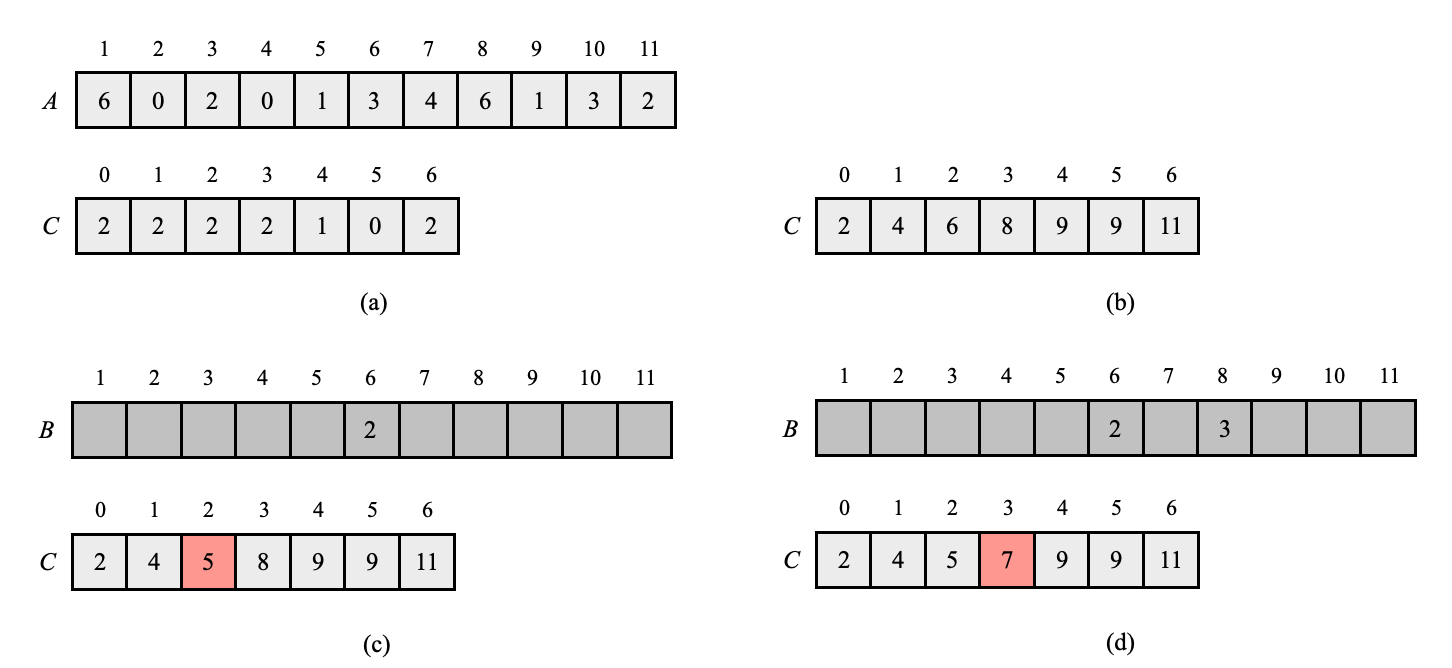
\includegraphics[scale=0.6]{hw3q3-1.png}

The diagram (a) demonstrates the resulting array C after recording occurrences of each distinct number in $A$. (b) updates $C$ such that it shows how many elements are less than or equal to $i$ in $C[i]$. Starting from (c), we iterate $A$ in reverse order. The first value to be handled is 2, which is at location $6$ according to $C$, so we simply put 2 at index 6 of $B$, and decrement its count in C. (d) shows $B$ and $C$ after 3, the next value in $A$, is processed. Following the same procedure, we can correctly arrange all the number from $A$ into $B$ shown below in (e) - (m).

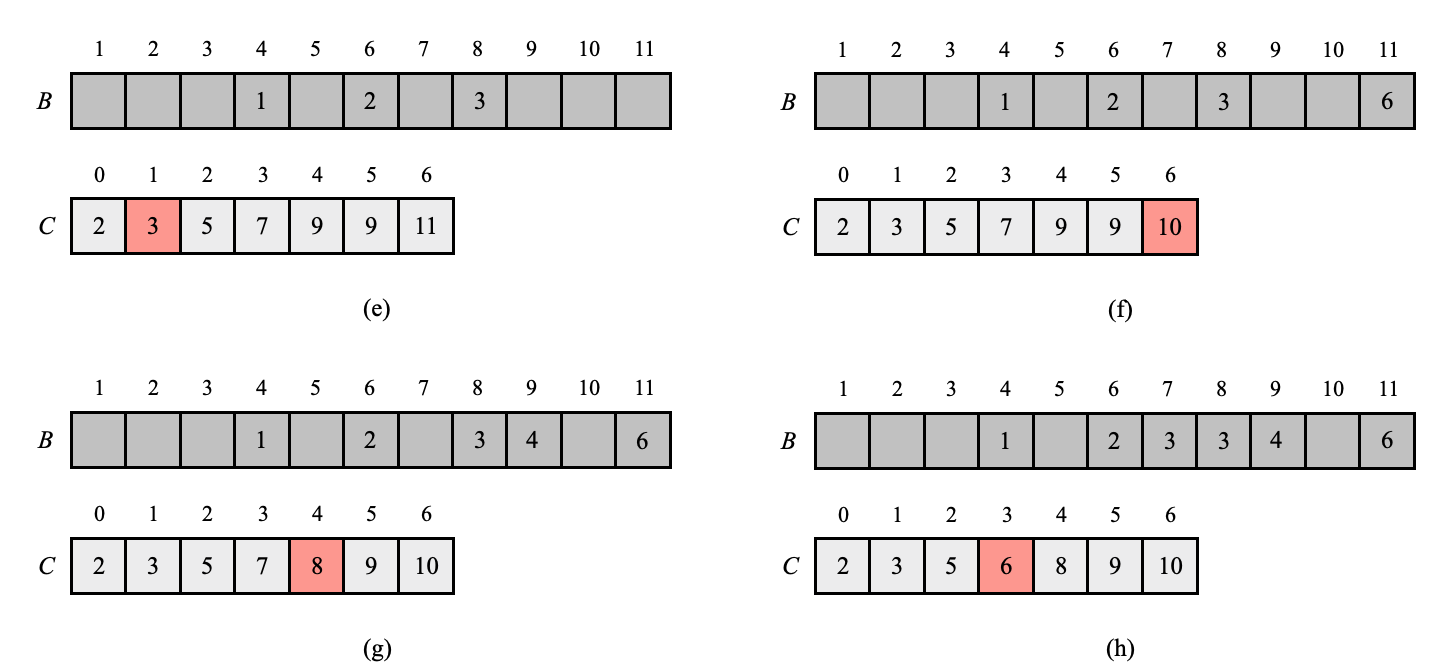
\includegraphics[scale=0.6]{hw3q3-2.png}

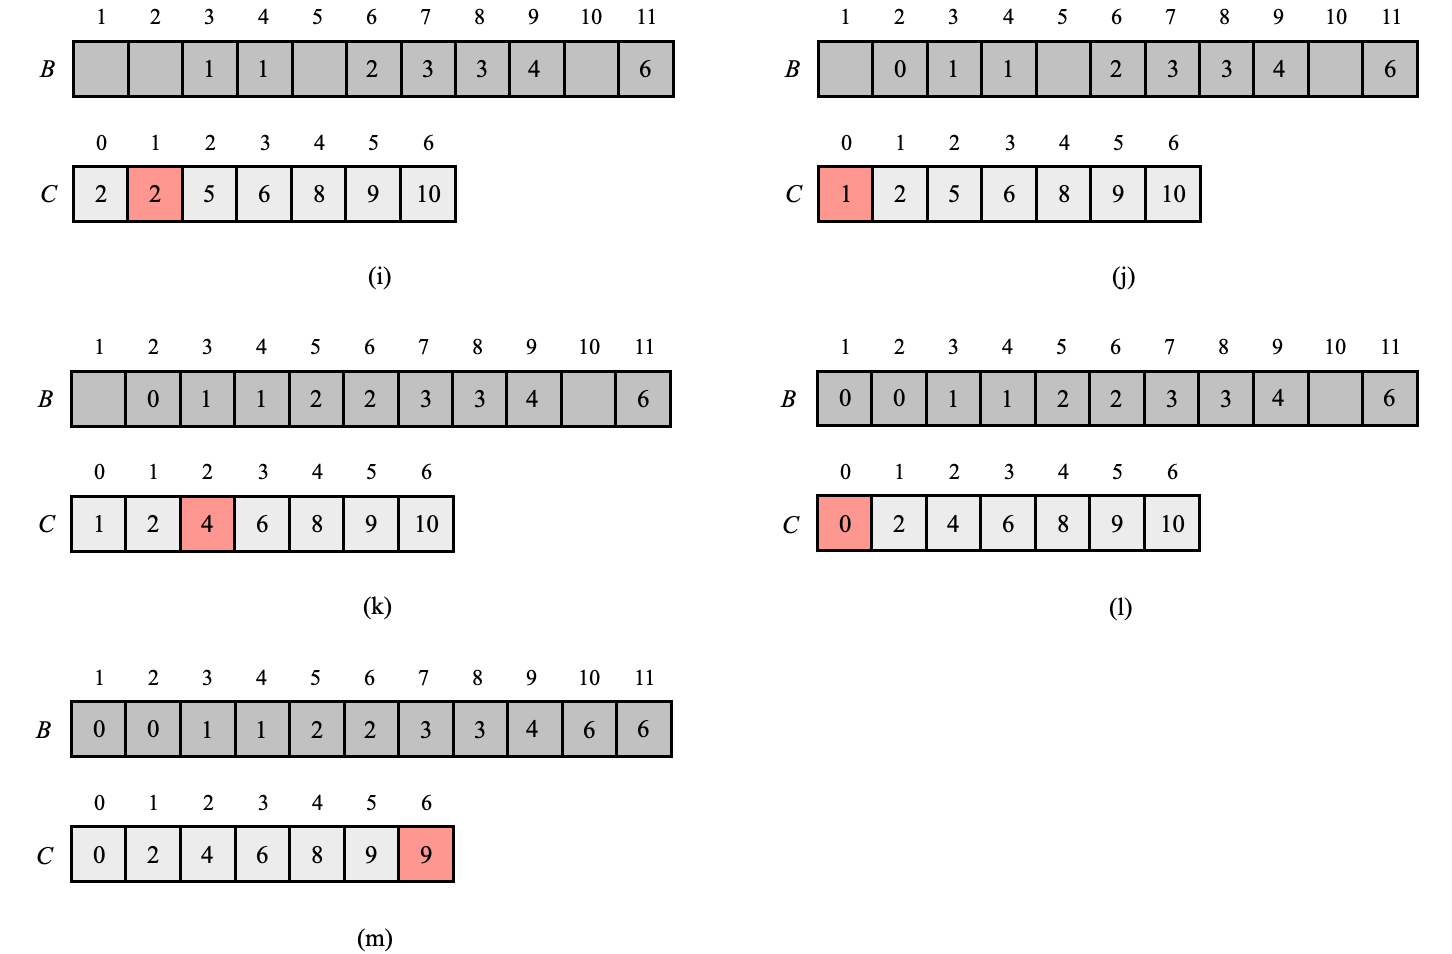
\includegraphics[scale=0.6]{hw3q3-3.png}

$B$ shows the final sorted array, $[0, 0, 1, 1, 2, 2, 3, 3, 4, 6, 6]$.


\newpage
%%% Problem 4 %%%
\begin{prob} \textbf{(5 points)} Exercise 8.2-4.
\end{prob}

Describe an algorithm that, given $n$ integers in the range $0$ to $k$, preprocesses its input and then answers any query about how many of the $n$ integers fall into a range $[a..b]$ in $O(1)$ time. Your algorithm should use $\Theta{(n+k)}$ preprocessing time.

\solution

The preprocessing step will be similar to how $\textproc{\textsc{Counting-Sort}}$ preprocesses values of an array. Specifically, the preprocessing consists of three steps. First, we initialize an array of $k+1$ number of zeros, $C$, where $k$ is the largest number found in the $n$ integers. Second, in $C$, we keep track of the occurrences of each distinct value while iterating through the $n$ integers. Third, we update $C$ such that $C[i]$ contains the number of elements less than or equal to $i$. The first step runs in $\Theta{(k)}$ time, the second step runs in $\Theta{(n)}$ time, and the third step runs in $\Theta{(k)}$ time. In total, the preprocessing takes $\Theta{(n+k)}$ steps. As a side note, in step 1, regardless of whether $k$ is given, we can find it in $O{(n)}$ time.

After the preprocessing, we could easily (in $O(1)$ time) answer the query by subtracting $C[b]$ with $C[a-1]$ because the number of elements less than or equal to $b$ is written in $C[b]$, and the number of elements less than or equal to $a$ is written in $C[a-1]$. Therefore, $C[b] - C[a-1]$ is just the number of elements that fall into the range $[a..b]$.


\newpage
%%% Problem 5 %%%
\begin{prob} \textbf{(5 points)} Exercise 8.3-1.
\end{prob}
Illustrate the operation of $\textproc{\textsc{Radix-Sort}}$ on the following list of English words: COW, DOG, SEA, RUG, ROW, MOB, BOX, TAB, BAR, EAR, TAR, DIG, BIG, TEA, NOW, FOX.

\solution

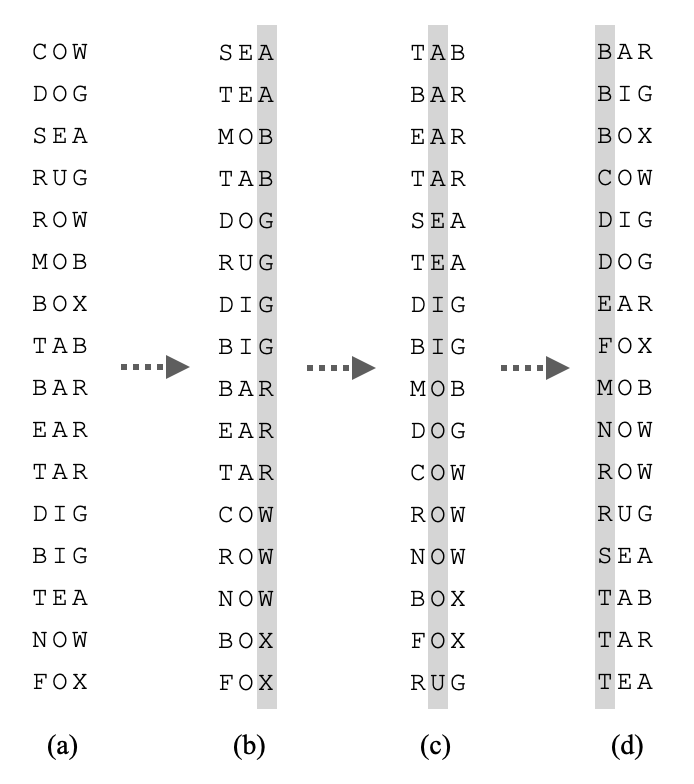
\includegraphics[scale=0.8]{hw3q5.png}

Radix sort processes from the least significant position to the most significant position, namely processing characters from right to left. Because each word has three characters, we can align them into columns as shown in (a). Words are sorted by alphabetical order by characters at column from right to left. (b) shows the result of sorting by the last column. (c) shows the result of sorting by the middle column, and (d) show the final sorted lists of words.


\newpage
%%% Problem 6 %%%
\begin{prob} \textbf{(10 points)} Exercise 8.3-3.
\end{prob}
Use induction to prove that radix sort works. Where does your proof need the assumption that the intermediate sort is stable?

\solution

\textbf{- Base case:} in the first iteration of the for loop (CLRS book 8.3 pseudocode), we sort the elements by the last digit, so we have the last 1 digit all sorted.

\textbf{- Inductive hypothesis:} assume that last $i$ digits are all sorted.

\textbf{- Inductive step:} at the $i+1$ iteration, a stable sort algorithm is applied to the array which sorts elements by the $i+1$ digit. For elements whose value at digit $i+1$ that are different, they will be arranged correctly by the sorting algorithm. On the other hand, for elements whose value at digit $i+1$ that are the same, their relative ordering is preserved thanks to the stable sort, which does not distinguish between values that are equal. In this case, by our hypothesis, the last $i$ digits are already sorted, so we know that the last $i+1$ digits are sorted.

At the last iteration, values are stably sorted by the most significant bit at which point we have all digits sorted. Hence we showed radix sort works by induction.


\newpage
%%% Problem 7 %%%
\begin{prob} \textbf{(5 points)} Exercise 8.3-4.
\end{prob}
Show how to sort $n$ integers in the range 0 to $n^3-1$ in $O(n)$ time.

\solution

The trick here is that we shall change each of the n integers from base 10 to base $n$. In this case, the largest value that a 1-digit base-n number can represent is $n-1$. The largest value that a 2-digit base-$n$ number can represent is $n^2 - 1$. The largest value that a 3-digit base-n number can represent is $n^3-1$. Because the largest possible value among the $n$ integers is $n^3-1$, there are two nice properties: every number can be represented using only 3 digits in a base-n number; the conversion of base operation can be done in constant time for every number. 

After this preprocessing, we can apply $\textproc{\textsc{Radix-Sort}}$ on the converted n number of base-n numbers. The runtime of  $\textproc{\textsc{Radix-Sort}}$ has been shown to be $\Theta{(d(n+k))}$ where $d$ is the number of digits, $n$ is the number of values to be sorted, and $k$ is the largest possible value for each digit. In this case, $d$ is a constant 3, and $k$ is just $n$ after the conversion. Therefore, we can sort in $\Theta{(3(n+n))} = \Theta{(n)}$. Because it's $ \Theta{(n)}$, it's also $O(n)$.


\newpage
%%% Problem 8 %%%
\begin{prob} \textbf{(20 points)} Exercise 9.1-1.
\end{prob}
Show that the second smallest of n elements can be found with $n + \lceil{\lg n}\rceil - 2$ comparisons in the worst case. (Hint: Also find the smallest element.)

\solution

The trivial solution results in $(n - 1) + (n - 1 - 1) = 2n - 3$ comparisons by first finding the smallest element and then finding the smallest element besides the element we just found. So, we need to resort to some ways to reduce the number of comparisons. 

The idea is that we consider elements in consecutive disjoint pairs, each of which has two elements i.e. comparing element at index $i$ with element at $i+1$ for i from 1 to $n-1$ with a $i$+=2 increment. We collect the smaller element in each pair, which results in $\lceil n/2 \rceil$ elements. We then perform the same procedure on the $\lceil n/2 \rceil$ number of smaller elements we just found. Applying this procedure $\lceil \lg n \rceil$ times, we find the smallest element. For the sake of the expressions' simplicity, we assume the number of inputs is power of 2  without loss of generality. The number of comparisons we have done here is: $n/2$ for the first run, $n/4$ for the second run, ..., and 1 for the last run. In total, there are $n-1$ comparisons needed to find the smallest element in this fashion,
\[
\begin{split}
\frac{n}{2} + \frac{n}{4} + \frac{n}{8} + \cdots + 1 &= \frac{n}{2} \sum_{i=0}^{\lg n} \frac{1}{2^i} \\
&= \frac{n}{2} \cdot \frac{1-\frac{1}{2}^{\lg n}}{1 - 0.5} \\
&= \frac{n}{2} \cdot \frac{1- n^{(\lg 1 - \lg 2)}}{0.5} \\
&= \frac{n}{2} \cdot \frac{1 - n^{-1}}{0.5} \\
&= n - 1
\end{split}
\]
Thanks to the procedure we performed, the smallest element must have been compared with the second smallest element once and won because the second smallest element could only be lost to the smallest element. To find it, this reminds us to keep track of whom is compared against in each comparison during the procedure of finding the smallest element. We know that the number of runs is bounded by $\lceil \lg n \rceil$, which means the smallest element have only been compared against $\lceil \lg n \rceil$ other elements. Finding the minimum among the $\lceil \lg n \rceil$ elements take $\lceil \lg n \rceil - 1$ comparisons. 

In summary, finding the smallest elements takes $n-1$ comparisons, and finding the second smallest takes $\lceil \lg n \rceil - 1$ comparisons. In total, we need $n - 1 + \lceil \lg n \rceil - 1 = n +  \lceil \lg n \rceil - 2$ comparisons to be exact to find the second smallest element.


\newpage
%%% Problem 9 %%%
\begin{prob} \textbf{(10 points)} Exercise 9.3-7.
\end{prob}
Describe an $O(n)$ time algorithm that, given a set $S$ of $n$ distinct numbers and a positive integer $k \le n$, determines the $k$ numbers in $S$ that are closest to the median of $S$.

\solution

As we know that $\textproc{\textsc{Select}}$ runs in $O(n)$ time in the worst case (CLRS 9.3), we use it to find $i$-th order statistics in our favor. The median resides in the half point, $n/2$, and its $k$ nearest neighbors reside between $n/2 - k/2$ and $n/2 + k/2$ positions. So, we first try to find the $(n-k)/2$-th order statistic in linear time. As a result, elements less than the $(n-k)/2$-th element are all on its left. Next, we find the $k$-th order statistic from the high side of the partition, which takes linear time. Then, elements greater than the $(n+k)/2$-th element are all on its right. Now, we can find those $k$ numbers that are closest to the median between $[(n-k)/2 ... (n+k)/2]$. We performed $\textproc{\textsc{Select}}$ two times, so the runtime is bounded by $2O(n) = O(n)$.


\newpage
%%% Problem 10 %%%
\begin{prob} \textbf{(20 points)} Exercise 9.3-8.
\end{prob}
Let $X[1..n]$ and $Y[1..n]$ be two arrays, each containing $n$ numbers already in sorted order. Give an $O(\lg n)$-time algorithm to find the median of all $2n$ elements in arrays $X$ and $Y$.

\solution

Because we have $2n$ elements, which is an even number, the median we discuss here will be the lower median, which is at index $\lfloor (2n+1)/2 \rfloor = \lfloor n + 1/2 \rfloor = n$. There are exactly $n-1$ elements to the left of the median and exactly $n$ elements to the right. We assert that the final median of all $2n$ elements reside between the median of $X$ and the median of $Y$ in the merged array. Let's prove this assertion in all cases:

- Case (1): when two medians are equal, the final median is trivially the median of $X$, which is at $\lfloor(n+1)/2 \rfloor$. We know that there are $\lfloor(n+1)/2 \rfloor - 1$ elements that are less than the final median in $X$, and the same happens in $Y$. When $n$ is odd, we have $2 \cdot ((n+1)/2 - 1) = n + 1 - 2 = n - 1$ elements less than or equal to the median. When $n$ is even, we have $2 \cdot (n/2 - 1) = n - 2$ elements less than the median. In addition, we know that there are at least two elements that equal to the final median. We can include one of them to the $n-2$ elements to make it that there exists $n-1$ elements to the left of the final median.

- Case (2): when the median of $X$ is less than that of $Y$, the final median should reside between the high partition of $X$ and the low partition of $Y$. We can prove this by contradiction. If the final median were to be in the lower partition of $X$, there would be \textbf{more than} $n/2$ elements in $X$ that are greater than the final median. Because the median of $Y$ is greater than that of $X$, there are also \textbf{more than} $n/2$ elements in $Y$ that are greater than the final median. In total, \textbf{more than} n elements are to the right of the final median, which contradicts the definition of a median in $2n$ elements. On the other hand, if the final median were to be in the high partition of $Y$, there would be \textbf{more than} $n/2$ elements that are smaller than the final median. As the median of $X$ is less than that of $Y$, there are \textbf{more than} $n/2$ elements that are smaller that the final median. In total, more than $n$ elements are to the left of the final median, which contradicts the definition of a median in $2n$ elements.

- Case (3): when the median of $X$ is greater than that of $Y$, the final median should reside between the low partition of $X$ and the high partition of $Y$. Similar to case (2), we can prove this is true by contradiction. Alternatively, we don't even need to prove it because $X$ and $Y$ are of same size, and they are just labels that won't make a difference for the final sorted array.

Now that we know our assumption is correct, we can write the pseudocode accordingly,
\begin{algorithmic}[1]
\Function{FindMedianSortedArrays}{\textit{nums1}, \textit{nums2}}
	\If {\textit{nums1}.length $\le 1$}
		\State \textbf{return} min(\textit{nums1}[0], \textit{nums2}[0])
	\EndIf
	\State $m = \text{Math.floor}((\textit{nums1}.length + 1)/2) - 1$
	\If {$\textit{nums1}[m] == \textit{nums2}[m]$}
		\State \textbf{return} $\textit{nums1}[m]$
	\EndIf
	\If {$\textit{nums1}[m] < \textit{nums2}[m]$}
		\State \textbf{return} $\textproc{\textsc{FindMedianSortedArrays}}(\textit{nums1}[m: ] \text{, }\textit{nums2}[:m+1])$
	\EndIf
	\State \textbf{return} $\textproc{\textsc{FindMedianSortedArrays}}(\textit{nums1}[:m+1] \text{, } \textit{nums2}[m:])$
\EndFunction
\end{algorithmic}


\newpage
%%% Problem 11 %%%
\begin{prob} \textbf{(15 points)} Exercise 9.3-9.
\end{prob}
Given the $x$- and $y$-coordinates of the wells, how should the professor pick the optimal location of the main pipeline, which would be the one that minimizes the total length of the spurs? Show how to determine the optimal location in linear time.

\solution

Since the main pipeline goes from east to west in a straight line, we couldn't use the least square method to fit a line that minimizes the total distance between each well and the fitted line. Instead, we want to find the median of the wells' y-coordinates in order to minimize the total length of the spurs. The median would be optimal because if we were to move the pipeline from the median up (north) by some amount $d$. Each distance from above the median would decrease by $d$; however, the distance below the median and including the median would be increased by $d$, which results in a longer total length. Similarly, the total length is higher if we move the main pipeline down (south) by some amount outside the median.

When the number of wells is odd, we can simply find the median of wells' y-coordinates to be the y-coordinate of the main pipeline using $\textproc{\textsc{Select}}$ which runs in linear time. 

When the number of wells is even, we can pick any value between the lower median at $i=\lfloor (n+1)/2 \rfloor$ and upper median at $i=\lceil (n+1)/2 \rceil$, which results in the same total length. Finding these $i$-th order statistics takes linear time.

In summary, we can determine an optimal location for the main pipeline in linear time.


\newpage
%%% Problem 12 %%%
\begin{prob} \textbf{(10 points)} Exercise 8.4-3.
\end{prob}
Let $X$ be a random variable that is equal to the number of heads in two flips of a fair coin. What is $\text{E}[X^2]$? What is $\text{E}^2[X]$?

\solution

For the random variable $X$, there are three cases: 0 head with probability 1/4; 1 head with probability 2/4; and 2 head with probability 1/4. Because it's a discrete random variable, we can compute the expectations using the formula $\text{E}[X] = \sum_i x_i p(x)$ where $x_i$ is the value of the random variable and $p(x)$ is the probability mass function.
\[
\text{E}[X^2] = 0^2 \cdot \frac{1}{4} + 1^2 \cdot \frac{1}{2} + 2^2 \cdot \frac{1}{4} = 0 + \frac{1}{2} + 1 = 1.5
\]

\[
\text{E}^2[X] = (0 \cdot \frac{1}{4} + 1 \cdot \frac{1}{2} + 2 \cdot \frac{1}{4})^2 = (0 + \frac{1}{2} + \frac{1}{2})^2 = 1
\]


\newpage
%%% Problem 13 %%%
\begin{prob} \textbf{(Extra credit 10 points)} Problem 9-1.
\end{prob}
\solution

%%% Problem 14 %%%
\begin{prob} \textbf{(Extra credit 20 points)} Problem 8-1.
\end{prob}
\solution

%%% Problem 15 %%%
\begin{prob} \textbf{(Extra credit 20 points)} Problem 8.4.
\end{prob}
\solution


\end{document}